% \setchapterimage[6cm]{seaside}
\setchapterpreamble[u]{\margintoc}
% \chapter{Defining a model of the implicit object construction}
\chapter{A Stochastic Optimality Theoretic account of object drop}
\labch{modeltheory}


% \section{Optimality Theories} \labsec{introtheory}

The model of the implicit object construction presented in this dissertation was developed under the Optimality Theory framework. In particular, it builds on the version of Stochastic Optimality Theory defined by \textcite{Medina2007} in order to model object drop in English.\\
In \refsec{classicot} I will present standard Optimality Theory and discuss both its strengths and its shortcomings. \refsec{harmonic_grammar} is devoted to Harmonic Grammar, the historical precursor of Optimality Theory, which is shown to possess attractive mathematical properties its descendant lacks, but also a number of problems making it a bad fit for modeling object drop. In \refsec{otgradience} I tackle the problem of moving from modeling the binary judgments traditionally used in syntax theory to modeling complex gradient judgments, which leads to the development of probabilistic grammars. A discussion of these and an in-depth introduction to Stochastic Optimality Theory are provided in \refsec{stochot}.

\section{Standard Optimality Theory} \labsec{classicot}

\subsection{Introduction} In \nrefch{factors}, the optionality of direct objects has been shown to depend on a large number of semantic, aspectual, and pragmatic factors. The challenge a linguistic model of object drop has to undertake is to account not only for the existence of relevant factors, but also for their combined effect on the grammaticality of the implicit object construction. My model will be based upon a probabilistic variant of Optimality Theory \parencite{princesmolensky1993optimality, PrinceSmolensky2008, PrinceSmolensky1997otIntro}. A full introduction to Optimality Theory and its intricacies goes well beyond the scope of this thesis, so I will only provide a short presentation to familiarize the reader with the framework and clarify its role in my research.\\ % 1. OPTIMALITY THEORY FOUNDATIONS
In a nutshell, the grammaticality of a linguistic structure in Optimality Theory is defined in terms of well-formedness with respect to a set of conflicting, re-rankable constraints. The constraints themselves are universal, while the order in which they are ranked is language-specific and determines the optimal (i.e., grammatical) output. Let us rephrase this in more technical, theory-specific terms. A grammar in Optimality Theory is built upon three components:
\begin{itemize}
    \item \textsc{\textbf{Gen}} is the function that generates candidate outputs based on the input provided. This function is unconstrained in its generative power, so that it can create any number and type of candidates by applying any operation, such as insertion and deletion, to the input (a property called "freedom of analysis"). Typically, software (such as OTSoft by \textcite{hayes2003otsoft} or SPOT by \textcite{bellik2019automated}) is used to trim the candidate set down to a feasible number of candidates to the optimization, since it would be time-prohibitive to do so by hand.
    \item \textsc{\textbf{Con}} is the set of universal, violable constraints, existing in two different kinds, whose ranking hierarchy makes up the grammar of a language. \textbf{Markedness} constraints force the output to satisfy some requirements, leading it to differ from the input depending on the specific requirement. \textbf{Faithfulness} constraints, on the contrary, require that the output be identical to the input and penalize any deviation. The conflict between markedness and faithfulness constraints is at the heart of Optimality Theory.
    \item \textsc{\textbf{Eval}} is the function that picks a winner among the candidates, based on the constraint ranking. In Standard Optimality Theory, the relation between any two constraints is one of \textit{strict domination}, meaning that the higher ranked constraint always dominates the lower ranked one regardless of how many violations each of them incurred in. As I will illustrate later in this Chapter, it is possible to define alternative versions of \textsc{\textbf{Eval}} in non-standard Optimality Theories where lower-ranked constraints can be more relevant than a higher ranked one based on their weights or violations.
\end{itemize}
Crucially, these three components are universal, i.e., they work the same in every language. The only language-specific aspect of an Optimality Theoretic grammar is the constraint hierarchy.\\
How does this work in practice? This question is best answered by looking at an example of the basic workings of Optimality Theory by \textcite{grimshaw1998optimal}, regarded as a classic model in the introduction to the use of the framework in syntactic theory by \textcite{legendre2001introduction}, and finally revised in \textcite{legendre2019otsyntax}. Optimality Theory itself was developed \parencite{princesmolensky1993optimality} within phonological theory, but in these pages I will only focus on its syntactic derivations. The version of the constraints and linguistic examples discussed in the next paragraph is the latest one by \textcite{legendre2019otsyntax}. 

\subsection{Optimality Theory in practice} A linguistic phenomenon often mentioned in textbooks is that languages allowing for topic-referring subjects to be dropped also require null expletives with weather verbs (as in \ref{ita_nullsubj}), while languages with compulsorily overt subjects require overt expletives with weather verbs (as in \ref{eng_nullsubj}).
\ex. \label{ita_nullsubj} Italian
\a. (Lui/Lei) ha mangiato tre panini.
\b. \label{ita_expletive} (*Esso) piove.

\ex. \label{eng_nullsubj} English
\a. *(She) has eaten three burgers.
\b. \label{eng_expletive} *(It) rains.

% COMPACT EXAMPLES AS IN https://www.ling.upenn.edu/~beatrice/syntax-textbook/glossary.html
In order to account for the difference between Italian and English with respect to their treatment of expletives, as shown in \ref{ita_expletive} and \ref{eng_expletive} respectively, the Optimalist has to individuate the relevant constraints populating \textsc{Con} and to set a conflict between them, i.e., to define them so that satisfying a constraint entails a violation of another.\\
In this case, only the two constraints in \ref{expletive_constraints} are at play. In particular, \textsc{Subject} \ref{expletive_subj} is the re-working of the Extended Projection Principle \parencite{chomsky1982epp} as a markedness constraint, while \textsc{Full-Int} \ref{expletive_fullint} is a faithfulness constraint capturing the Principle of Full Interpretation \parencite{chomsky1991fullint}.
\ex. \label{expletive_constraints} \a. \label{expletive_subj} \textsc{Subject}: The subject surfaces in SpecTP.
\b. \label{expletive_fullint} \textsc{Full-Int}(erpretation): Lexical items contribute to the interpretation of a structure.

\textsc{Subject} and \textsc{Full-Int} are in conflict in the case of zero-argument verbs (such as weather verbs) because satisfying the former requires the use of an overt expletive, which is forbidden by the latter, while satisfying \textsc{Full-Int} requires a null expletive, which goes against \textsc{Subject}. No sentence can possibly satisfy both constraints at the same time. Conflicts in Optimality Theory are solved by re-ranking the constraints based on the violations each competing candidate incurs into.\\
Let us discuss the tableaux for Italian and English weather verbs, in \reftab{tableau_ita_expletive} and \reftab{tableau_eng_expletive} respectively, where the competition between candidates and its outcome are made esplicit.

\begin{table}[htb] % the "htb" makes table env unfloaty
\caption{Optimality Theoretic tableau for weather verbs in Italian.}
\labtab{tableau_ita_expletive}
\begin{tabular}{|ll|c|c|}\hline   
      & \textbf{\textit{piovere}\textsubscript{v}[present]}  & \textsc{Full-Int}  &  \textsc{Subject}\\ \hline\hline
      & a. EXPL piove     & *!         &           \\ \hline
\hand & b. piove     &            & *       \\ \hline
\end{tabular}
\end{table}

\begin{table}[htb] % the "htb" makes table env unfloaty
\caption{Optimality Theoretic tableau for weather verbs in English.}
\labtab{tableau_eng_expletive}
\begin{tabular}{|ll|c|c|}\hline   
      & \textbf{\textit{rain}\textsubscript{v}[present]}  & \textsc{Subject}  &  \textsc{Full-Int}\\ \hline\hline
\hand      & a. EXPL rains     &           & *         \\ \hline
 & b. rains     & *!           &       \\ \hline
\end{tabular}
\end{table}

The input to syntactic optimization in Optimality Theory contains only the relevant semantic information (lexical items, argument structures, and tense specifications), and all competitors share the same semantic content. In our case, the input contains the verb, its tense, and no argument structure since weather verb have no thematic arguments. Crucially, the expletive subject is not part of the input. Instead, it is supplied to a candidate output by \textsc{Gen}, the Generator function mapping the input to the set of all possible candidates to the optimization, i.e., mapping the propositional content of the input to all possible surface forms in the output. The resulting set comprises two candidates, one with an expletive subject (in $a.$) and one without (in $b.$). As explained above, candidates with an expletive subject violate \textsc{Full-Int} and subject-less candidates violate \textsc{Subject}. In the tableaux, an asterisk marks a violation of a constraint, an exclamation mark after an asterisk marks a \textit{fatal} violation (i.e., a violation excluding the candidate from further evaluation), the pointing finger indicates the optimal candidate, and constraints are ordered so that each constraint dominates the one to its right. Given the typology sketched in \ref{ita_expletive} and \ref{eng_expletive}, an Optimality Theoretic analysis of Italian and English leads to the conclusion that the difference between the two languages with respect to zero-argument verbs results from the different ranking of two universal constraints, \textsc{Full-Int} and \textsc{Subject} (as shown in the tableaux  \reftab{tableau_ita_expletive} and \reftab{tableau_eng_expletive}).\\
An explanation of the behavior of weather verbs in Italian and English, as well as a broader account of the typology in \ref{ita_nullsubj} and \ref{eng_nullsubj}, is not something that can happen only under Optimality Theory. For instance, Principles-and-Parameters theory accounts for the different behavior of Italian and English with the \textsc{Pro-Drop} parameter, so that Italian is a [+pro-drop] language and English is a [-pro-drop] language. In such a framework, inviolable, fixed parameters determine the grammaticality of a linguistic structure in a given language. Optimality Theory on the contrary, as "a formal theory of constraint interaction in Universal Grammar" \parencite{legendre2001introduction} relies on violable, re-rankable constraints to determine grammaticality. Most importantly, grammaticality is given to a linguistic structure as the outcome of a competition among several candidates, instead of being a property of that linguistic structure taken on its own. This is a crucial aspect of Optimality Theory that makes it a suitable framework for my analysis of the implicit object construction, even though \textit{standard} Optimality Theory suffers from problems that are best solved by other variants of the same framework. % 5. Kuhn's examples against standard OT
\subsection{Impossible violation profiles} To explain the nature of these problems, I will start with an example. Let us say that we collected a small set of data from a single language, that we wanted to model the distribution of these data using three theory-driven constraints, and that these data presented the constraint violation profiles represented in \reftab{tableau_kuhn_1}, \reftab{tableau_kuhn_2}, and \reftab{tableau_kuhn_3}.

\begin{table}[htb] % the "htb" makes table env unfloaty
\caption{Hypothetical Optimality Theoretic tableau for mock data by \textcite{kuhn2002corpus}}
\labtab{tableau_kuhn_1}
\begin{tabular}{|ll|c|c|c|}\hline   
      & \textbf{(a) candidate set:}  & \textsc{Constr. 3}  &  \textsc{Constr. 1} & \textsc{Constr. 2}\\ \hline\hline
\hand      & candidate A     &           & *         & * \\ \hline
 & candidate B     & ***           &       & \\ \hline
\end{tabular}
\end{table}

\begin{table}[htb] % the "htb" makes table env unfloaty
\caption{Hypothetical Optimality Theoretic tableau for mock data by \textcite{kuhn2002corpus}}
\labtab{tableau_kuhn_2}
\begin{tabular}{|ll|c|c|c|}\hline   
      & \textbf{(b) candidate set:}  & \textsc{Constr. 1}  &  \textsc{Constr. 2} & \textsc{Constr. 3}\\ \hline\hline
\hand      & candidate A'     &           &          & * \\ \hline
 & candidate B'     &            & *      & \\ \hline
\end{tabular}
\end{table}

\begin{table}[htb] % the "htb" makes table env unfloaty
\caption{Hypothetical Optimality Theoretic tableau for mock data by \textcite{kuhn2002corpus}}
\labtab{tableau_kuhn_3}
\begin{tabular}{|ll|c|c|c|}\hline   
      & \textbf{(c) candidate set:}  & \textsc{Constr. 1}  &  \textsc{Constr. 2} & \textsc{Constr. 3}\\ \hline\hline
\hand      & candidate A''     &           &          & * \\ \hline
 & candidate B''     & *           &       & \\ \hline
\end{tabular}
\end{table}

It is evident that this model of our mock data is unfeasible, considered that in any given language the constraints have to be ordered consistently (under the assumption of strict dominance). However, in the model above this does not happen, since \reftab{tableau_kuhn_1} is a ranking argument for \textsc{Constr. 3} $\gg$ \textsc{Constr. 1} and \textsc{Constr. 3} $\gg$ \textsc{Constr. 2}, while \reftab{tableau_kuhn_2} and \reftab{tableau_kuhn_3} are ranking arguments for the opposite.\\
It is possible that these constraints have to be ditched in favor of a whole new set of constraints, but let's say they are very well motivated by literature on the topic and there is no reason in linguistic theory to doubt their effect on the grammaticality of these data. Another possible solution to the inconsistency would be to introduce an additional constraint, \textsc{Constr. 4}, which would be ranked higher than all the others and violated only by candidate B. Provided we could indeed find such a constraint, this would lead to a situation where all the candidate sets from this hypothetical language are consistent with the ordinal constraint ranking \textsc{Constr. 4} $\gg$ \textsc{Constr. 1} $\gg$ \textsc{Constr. 2} $\gg$ \textsc{Constr. 3}. Yet, \textsc{Constr. 4} may be weakly grounded in the linguistic theory and thus a poor choice for a constraint in an Optimality Theoretic analysis. Remember that constraints are assumed to be part of Universal Grammar, and they have to be ranked consistently within a given language. What if \textsc{Constr. 4} is found to be incompatible with newer data from the same hypothetical language considered above? The quest to find an additional suitable constraint could continue, but the same problem would surface again and soon lead to an unmotivated number of constraints. I will provide a possible solution to this problem (and discuss its shortcomings) in \refsec{harmonic_grammar}. % 2. OT RELIES ON BINARY JUDGMENTS AND THEY ARE BAD FOR OBJ DROP

\subsection{Why standard OT is a bad fit for a model of object drop} \labsec{ot_bad_dobjdrop}
I will now focus on a feature of standard Optimality Theory that, while not being a worrying issue \textit{per se}, may become a problem for those using it to model a phenomenon as complex as that of indefinite object constructions. Let us see why.\\
Linguists adopting standard Optimality Theory to perform their analyses of syntax and other aspects of grammar rely on binary grammaticality judgments. As illustrated above, given a set of candidates competing for optimality, the optimization yields only one optimal candidate, which is the only candidate deemed grammatical, while all the others are equally ungrammatical regardless of the number or ranking of constraint violations they incurred into. Now, considering the phenomenon examined in this dissertation, a traditional Optimality Theoretic approach to modeling the grammaticality of the implicit object construction would only account for an oversimplified typology such as the one in \ref{naive_objdrop}. 
\ex. \label{naive_objdrop} \a. \label{naive_objdrop_sing} John sang.
\b. \label{naive_objdrop_build} *John built.

Such an account would perfectly describe a world where the linguistic factors presented in \nrefch{factors} make some object-less sentences with transitive verbs fully grammatical (as in \ref{naive_objdrop_sing}) and other ones fully ungrammatical (as in \ref{naive_objdrop_build}). However, the actual scenario is more complex. For instance, a classic Optimality Theoretic analysis of object drop would not capture the different grammaticality of the sentences in \ref{mature_objdrop_eat}, even though the literature suggests the imperfective sentence should be at least slightly more acceptable than the sentence in the perfective aspect. Similarly, it would fail to model cases such as \ref{mature_objdrop_build}, where neither candidate is fully grammatical, making it weird, if not altogether wrong, to declare an \textit{optimal} candidate.
\ex. \label{mature_objdrop_eat} \a. John had eaten.
\b. John was eating.

\ex. \label{mature_objdrop_build} \a. *John built.
\b. \textsuperscript{?}John was building again.

Example \ref{failot_medina} is the one used by \textcite[62]{Medina2007} to make the point that, crucially, the grammaticality of indefinite object drop varies not only within a group of candidates featuring the same verb, but also across verbs.
\ex. \label{failot_medina} \a. Jack ate.
\b. *Jack found.
\c. \textsuperscript{?}Jack caught.

Standard Optimality Theory fails to capture all of these observations in a viable model of object drop. I will discuss possible solutions to this problem in \refsec{otgradience} and focus on the one I will use for my experiments in \refsec{stochot}. In particular, I will make it clear that a model is necessary which accounts for nuanced, gradient effects \textemdash a goal that is unattainable within the realm of standard Optimality Theory.\\
Indeed, the standard Optimality Theoretic model of indefinite object drop in English devised by \textcite{yankes2021objectdropot} suffers from these exact problems. The author acknowledges the concerns relative to the glaringly obvious \textit{gradient} grammaticality of the implicit indefinite object construction, but dismisses them by simply stating that whenever his model chooses the null-object candidate as a winner over the overt-object candidate, this has to be interpreted as a possibility available in the grammar, rather than a strict imposition. On the contrary, he argues that the grammar would never allow for object drop in all the cases where the winner is the overt-object candidate. This explanation serves well a model entrenched in standard Optimality Theory, but, to a closer analysis, it appears to be an attempt to run with the hares and hunt with the hounds. Given the existence of well-known strategies to model linguistic phenomena showing unmistakable gradient grammaticality (both within and without the realm of Optimality Theory, as discussed in \refsec{weightedot}), it makes little sense to resort to a theory of grammar where only one winner candidate is possible, only to admit unquantified gradience in some cases. The author claims to be "seeking to apply the concepts of Optimality Theory to a new space", perhaps laying "the groundwork for a more rigorous overhaul in the future", but in doing so he overlooks the gradient, probabilistic model of indefinite null objects in English devised by \textcite{Medina2007} within the framework of (stochastic) Optimality Theory. I will come back to this in \refch{medina}.


\section{Weighted approaches to constraint ranking} \labsec{weightedot}

\subsection{Harmonic Grammar} \labsec{harmonic_grammar} % 6. Kuhn's examples introducing Harmonic Grammar
Let us forgo standard Optimality Theory and try replacing ranked ordinal constraints with numerically weighted ones, to avoid resorting to additional constraints and solve the problem of having impossible violation profiles. 
This was actually the strategy employed by the historical precursor of Optimality Theory, Harmonic Grammar, sketched out by \textcite{smolensky1993integrating, legendre1990can, legendre1991unifying} and later discussed in the light of Optimality Theory by \textcite{legendre2006optimality, pater2009weighted}. Harmonic Grammar was created as an attempt to bridge the apparently insurmountable gap between generative grammar, which is a formal model of existing languages, and linguistic models based on connectionism, which are instead models of cognition translating the patterns of neural activity into mathematical functions. Most importantly, there is no notion of constraint \textit{ranking} in Harmonic Grammar, so that their ordered depiction in tableaux has no bearing on the model itself.\\
In practice, Harmonic Grammar models assign a non-negative numerical weight to each constraint, each candidate gets a negative score for each violation of a constraint or a positive score for each satisfaction (unlike in Optimality Theory), and the harmony of each candidate is computed as in \refeq{harmony}. 

\begin{equation} \labeq{harmony} % formula in Pater (2009: 1006)
H = \sum_{k=1}^{K} s\textsubscript{k} w\textsubscript{k}
\end{equation}

Given a set of $k$ constraints, s\textsubscript{k} is the violation score of a candidate and w\textsubscript{k} is the weight of a constraint. The only candidate deemed grammatical, i.e., the winner of the competition for optimality, is the most harmonic in the candidate set. Unlike in Optimality Theory, where strict domination determines that the violation of a higher-ranked constraint is always worse than the violation of a lower-ranked constraint, the weighting of constraints in Harmonic Grammar makes it possible to model the cumulative effect of multiple violations of a constraint (see \reftab{hg_kuhn_1}). \\
Let us look at some made-up examples in \reftab{hg_kuhn_1}, adapted from Example 7 in \textcite{kuhn2002corpus} to conform to Harmonic Grammar symbolism. Unlike tableaux in Optimality Theory, Harmonic Grammar tableaux have an additional row for constraint weights and an additional column for the harmony scores of candidates. The starting weights assigned to the three constraints in the examples below do not determine a reliable model, since they are compatible with the candidate sets (a) and (b), but not with (c), where candidate B results more harmonic than candidate A.  Based on \refeq{harmony}, the harmony of each candidate is computed by multiplying each violation score by the weight of the violated constraint (e.g., -1*4 = -4 and -1*1 = -1 in (a)) and the summing up these partial results (in (a), -4 + (-1) = -5). Within a tableau, the grammatical candidate is the most harmonic, i.e., the one with the highest harmony value (in (a), this is candidate A, since -5 is bigger than -9). Thus, the starting weights are incompatible with (c), where the grammatical candidate has a lower harmony score than the other one (-3 is smaller than -1).


\begin{table}[htb] % the "htb" makes table env unfloaty
\caption{Hypothetical Harmonic Grammar tableaux for mock data, adapted from \textcite{kuhn2002corpus}}
\labtab{hg_kuhn_1}
\begin{tabular}{|ll||c|c|c||c|}\hline   
      & \textbf{(a) candidate set:}  & \textsc{\rotatebox[origin=c]{90}{ Constr. 1 }}  &  \textsc{\rotatebox[origin=c]{90}{ Constr. 2 }} & \textsc{\rotatebox[origin=c]{90}{ Constr. 3 }} & \textit{H}\\
       &  & 4 & 3 & 1 & \\
      \hline\hline
\hphantom{??? } \hand      & candidate A     & -1          &          & -1 & -5 \\ \hline
 & candidate B     &            & -3      & & -9\\ \hline
\end{tabular}
% \end{table}

\vspace*{0.5 cm}

% \begin{table}[htb] % the "htb" makes table env unfloaty
% \caption{Hypothetical Harmonic Grammar tableau for mock data, adapted from \textcite{kuhn2002corpus}}
% \labtab{hg_kuhn_2}
\begin{tabular}{|ll||c|c|c||c|}\hline   
      & \textbf{(b) candidate set:}  & \textsc{\rotatebox[origin=c]{90}{ Constr. 1 }}  &  \textsc{\rotatebox[origin=c]{90}{ Constr. 2 }} & \textsc{\rotatebox[origin=c]{90}{ Constr. 3 }} & \textit{H}\\
       &  & 4 & 3 & 1 & \\
      \hline\hline
\hphantom{??? } \hand      & candidate A'     &           & -1         &  & -3 \\ \hline
 & candidate B'     & -1           &       &    & -4\\ \hline
\end{tabular}
% \end{table}

\vspace*{0.5 cm}

% \begin{table}[htb] % the "htb" makes table env unfloaty
% \caption{Hypothetical Harmonic Grammar tableau for mock data, adapted from \textcite{kuhn2002corpus}}
% \labtab{hg_kuhn_3}
\begin{tabular}{|ll||c|c|c||c|}\hline   
      & \textbf{(c) candidate set:}  & \textsc{\rotatebox[origin=c]{90}{ Constr. 1 }}  &  \textsc{\rotatebox[origin=c]{90}{ Constr. 2 }} & \textsc{\rotatebox[origin=c]{90}{ Constr. 3 }} & \textit{H}\\
       &  & 4 & 3 & 1 & \\
      \hline\hline
??? \hand      & candidate A''     &           & -1         &  & -3 \\ \hline
 & candidate B''     &            &       & -1   & -1\\ \hline
\end{tabular}
\end{table}

The optimization process in this Harmonic Grammar model of our mock data has to continue, by means of updating the weight of each constraint via backpropagation\sidenote{Backpropagation is a resource-intensive training algorithm. Linear Optimality Theory, a later update of Harmonic Grammar, determines constraint weights using instead standard least square estimation (and only models violations, not satisfactions, of constraints).} until the model converges on a consistent representation of linguistic data. Interested readers who want to try their hand at this will find that the intended configuration would be $w_1$ = 6, $w_2$ = 4, $w_3$ = 5. At first glance, it would indeed seem that a simple computation saved us the trouble of coming up with unmotivated constraints, and yielded the intended model of our linguistic data. However, as \textcite{kuhn2002corpus} puts it, a weighted-constraint theory has an "undesiderable property" for the linguist trying to model typologically realistic languages with linguistically motivated constraints. Indeed, in Harmonic Grammar the linguistic motivation of a set of constraints risks being trivial, since it is always possible to bend the weight set until the model accomodates all data, regardless of the constraints used in the model. A severe consequence of this state of affairs is that Harmonic Grammar (or any other version of an Optimality Theoretic-like grammar with weighted constraints) overgenerates data, namely, it predicts both possible and impossible languages \parencite{legendre2006optimality, pater2009weighted}.\\
Harmonic Grammar, at least in its original formulation, is a very powerful connectionist tool, but a poor model of the actual typology of human languages. \textcite[216]{princesmolensky1993optimality} thus conclude that "recourse to the full-blown power of numerical optimization is not required", a concept that has become famous among linguists in its witty form "grammars don't count", and further explored in \textcite{smolensky2006harmony}. Optimality Theory was then developed as a more restricted, linguistically motivated spawn of Harmonic Grammar, which replaces weighted constraints with constraints ranked according to strict dominance. Optimality Theory is the last step in the path towards symbolic functions and representations that started with fully numerical neural networks and continued with functionally numerical but representationally symbolic Harmonic Grammar. It is important to observe that the weighting-to-ranking shift still has a clear mathematical meaning, which becomes apparent if one were to recast an Optimality Theoretic analysis in an Harmonic Grammar fashion. From this perspective, strict dominance can be seen as the result of exponential weighting of the constraints (so that no violation profile can exist where a lower-ranked constraint outranks a higher-ranked constraint), making Optimality Theory "a very specialized kind of Harmonic Grammar" \parencite{princesmolensky1993optimality, PrinceSmolensky2008}. Thus, Optimality Theory is the actual intended link between generative grammar and neural computation, being a formal theory of constraint interaction (i.e., Universal Grammar) grounded in empirical observations about language and connectionist math. However, neither Harmonic Grammar nor standard Optimality Theory are the most suitable framework to model gradient judgments about the implicit object construction.


\subsection{Going gradient} \labsec{otgradience} % 3. KELLER'S EXTENDED OT HAS SUBOPTIMALITY FOR GRADED, DISCRETE JUDGS
As we saw, a phenomenon as complex as indefinite object drop can't possibly be described by means of binary grammaticality judgments. \textit{Gradient} judgments\sidenote{For observations on the importance of gradient acceptability judgments for linguistic theory beyond Optimality Theory, as well as some words of caution pertaining their validity, please refer to \textcite{Schutze2016, rimmer2006grammaticality, BornkesselSchlesewsky2007, Sprouse2007, JuzekHaussler, LauEtAl2017}.} have to be collected instead, and a linguistic model has to be created to account for \textit{gradient} grammaticality.\\
A first attempt to bridge the gap between the resources of standard Optimality Theory and the need for finer-grained acceptability judgments was made by \textcite{keller1997extraction}. In this work, the assumption of standard Optimality Theory that all non-optimal candidates are equally ungrammatical is dropped, in favor of an extended version of the framework where the grammaticality of each candidate is formulated in terms of a relative rank with respect to its competitors. While in standard Optimality Theory grammaticality equates to \textit{global} optimality over the whole candidate set, in Extended Optimality Theory it equates to \textit{local} optimality with respect to a subset of the candidate set (aptly named "suboptimality"). Extended Optimality Theory thus establishes a grammaticality hierarchy among the candidates, and this predicted hierarchy can be evaluated against empirical data, i.e., graded acceptability judgments.\\
Let us look at an example from Keller's experiment on the effect of definiteness and verb class on extraction from verbs \parencite[10-12]{keller1997extraction}. The acceptability judgments he obtained\sidenote{Mean acceptability ratings obtained via a magnitude estimation experiment \parencite{bard1996magnitude} involving nineteen native speakers of English.} for the sentences in \ref{keller1997_sentences} show that extraction from \textit{take}-type verbs is more acceptable than extraction from \textit{destroy}-type verbs, that the extraction of indefinite arguments is more acceptable than the extraction of definite arguments, and that verb class has a stronger effect than definiteness on grammaticality.
\ex. \label{keller1997_sentences} \a. Which man did you take a picture of? \hfill 49.39
\b. Which man did you take the picture of? \hfill 43.74
\c. Which man did you destroy a picture of? \hfill 41.01
\d. Which man did you destroy the picture of? \hfill 36.94

The Extended Optimality Theoretic tableaux representing the violation profiles of these candidates is in \reftab{keller1997_tableau}. \textcite{keller1997extraction} bases his choice of constraints on \textcite{diesing1992indefinites}, \textcite{legendre1995optimality}, and \textcite{legendre1998less}, which I won't discuss here in full length due to space constraints. The \textsc{Bar}\textsuperscript{\textit{n}} constraints are an implementation of the \textsc{MinimalLink} family of constraints, which requires chain links\sidenote{When a constituent moves in a syntax tree, chains are the combination of the moved copy and the trace it leaves behind.} to cross a minimal amount of barriers (see \textcite{chomsky1993minimalist} for a full explanation of the Minimal Link Condition, according to which syntactic movement has to target the closest potential landing site). \textsc{Bar} has a counter for each time a barrier gets crossed. \textsc{SubCat} requires instead that subcategorization requirements be met. The syntactic representation of each candidate in \reftab{keller1997_tableau} follows directly from the theory of extraction by \textcite{legendre1995optimality} and \textcite{legendre1998less}, and from the theory of definiteness by \textcite{diesing1992indefinites}, which requires that [-creation] verbs such as 'to destroy' subcategorize for a definite NP. M is a mapping operator correlating with the definiteness feature, and it turns the projection it adjoins to into a barrier for movement (more on this in \textcite[11]{keller1997extraction} and literature referenced hereby).\\
Let us comment the violation profiles in the tableau. All candidates violate \textsc{Bar\textsuperscript{1}} once because the chain $\langle M\textsubscript{j}, NP\textsubscript{j} \rangle$ crosses the barrier VP. The chain $\langle \text{which man}\textsubscript{i}, t\textsubscript{i} \rangle$ crosses only VP in candidate (a), resulting in another violation of \textsc{Bar\textsuperscript{1}}, while it crosses both VP and IP (made into a barrier by M) in candidate (b), resulting in a violation of \textsc{Bar\textsuperscript{2}}. \textcite{keller1997extraction} comments that the additional violation of \textsc{Bar\textsuperscript{n}} candidates (c) and (d) incur into is due to the fact that barrierhood correlates with feature selection, so that a definiteness feature requirement on the verb turns it into an additional barrier for the movement. Candidate (c) also violates \textsc{SubCat} because the [-creation] verb subcategorizes for an indefinite NP.

\begin{table}[htb] % the "htb" makes table env unfloaty
\caption{Extended Optimality Theory tableau relative to the examples in \ref{keller1997_sentences}, from \textcite[12]{keller1997extraction}.}
\labtab{keller1997_tableau}
\begin{adjustbox}{max width=\textwidth}
\begin{tabular}{|ll||c|c|c|c|}\hline   
      & \textbf{Q\textsubscript{\textit{i}} [NP\textsubscript{Subj} V [NP\textsubscript{Pict} \textit{x\textsubscript{i}}[+wh]]}  & \textsc{\rotatebox[origin=c]{90}{ Bar }}  &  \textsc{\rotatebox[origin=c]{90}{ SubCat }} & \multicolumn{2}{|c|}{\textsc{Bar}}\\
       &  & 3 &  & 2 & 1 \\
      \hline\hline
\hand a.      & \vtop{\hbox{\strut [\textsubscript{CP} which man\textsubscript{\textit{i}} did [\textsubscript{IP} you [\textsubscript{VP} M\textsubscript{\textit{j}} [\textsubscript{VP} take}\hbox{\strut [\textsubscript{NP \textit{j} [-def]} a picture of t\textsubscript{\textit{i}}[+wh]]]]]]}}     &           &          &  & ** \\ \hline
b. & \vtop{\hbox{\strut [\textsubscript{CP} which man\textsubscript{\textit{i}} did [\textsubscript{IP} M\textsubscript{\textit{j}} [\textsubscript{VP} you [\textsubscript{VP} take}\hbox{\strut [\textsubscript{NP \textit{j} [+def]} the picture of t\textsubscript{\textit{i}}[+wh]]]]]]}}     &            &   & * & *\\ \hline
c. & \vtop{\hbox{\strut [\textsubscript{CP} which man\textsubscript{\textit{i}} did [\textsubscript{IP} you [\textsubscript{VP} M\textsubscript{\textit{j}} [\textsubscript{VP} destroy\textsubscript{[+def]}}\hbox{\strut [\textsubscript{NP \textit{j} [-def]} a picture of t\textsubscript{\textit{i}}[+wh]]]]]]}}     &            & * & * & *\\ \hline
d. & \vtop{\hbox{\strut [\textsubscript{CP} which man\textsubscript{\textit{i}} did [\textsubscript{IP} M\textsubscript{\textit{j}} [\textsubscript{VP} you [\textsubscript{VP} destroy\textsubscript{[+def]}}\hbox{\strut [\textsubscript{NP \textit{j} [+def]} the picture of t\textsubscript{\textit{i}}[+wh]]]]]]}}     &  *      &   &  & *\\ \hline
\end{tabular}
\end{adjustbox}
\end{table}

The constraint ranking in \reftab{keller1997_tableau} is compatible with the grammaticality judgments in \ref{keller1997_sentences}. Supported by empirical data, this Optimality Theoretic analysis does more than yield a single optimal candidate. As a matter of fact, it predicts a grammaticality hierarchy by exploiting evidence from the optimal candidate and the suboptimal ones alike. Candidate (a) is the optimal candidate, the one which would stand out as the only winner in a standard Optimality Theoretic analysis. Candidate (b) is suboptimal, in that it violates a higher-ranked constraint than (a), but it still performs better than (c). The same goes for candidates (c) and (d), each showing decreasing degrees of optimality based on their violation profiles.\\
An important consequence of predicting \textit{sub}optimality in place of plain optimality is that such an analysis makes a stronger case for a given constraint ranking, given that re-ranking a constraint may not affect the optimal candidate, but it may have visible effects on suboptimal candidates. For instance, re-ranking \textsc{SubCat} over \textsc{Bar\textsuperscript{3}} in \reftab{keller1997_tableau} would not affect the optimality of candidate (a.), but it would wrongly make candidate (d.) more suboptimal than (c.). Thus, Extended Optimality Theory leverages the same features of the standard framework, but is also able to detect otherwise hidden re-rankings and to include finer-grained grammaticality judgments in the linguistic analysis.\\
Nevertheless, while this extension of the original framework makes it possible for syntacticians to model non-binary grammaticality judgments, it does not go beyond the assumption of strict domination among constraints. Moreover, even though graded grammaticality judgments are collected from native speakers and averaged to evaluate the (sub)optimality of candidates, these numerical values have only ordinal meaning. In other words, they are used to rank the candidates according to their grammaticality, but they have no other use. As a result, in Extended Optimality Theory the gradience of grammaticality actually stems from discrete, not continuous, values.

\subsection{Probabilistic grammar} \labsec{probgrammar} % 4. LITTLE INTRO TO STOCHASTIC THEORIES
Looking at the bigger picture of what rippled through linguistics at the turn of the century, awareness of the aforementioned issues with Optimality Theory (and its precursor, and its early extension) went hand in hand with a growing discontent with the many limits of traditional linguistic theories based on categorical definitions and binary judgments. The road that took linguists from a categorical view of language to modeling gradient grammaticality was a long, bumpy one. Ever since \textcite{chomsky1957syntactic} frowned upon the notion of "probability of a sentence", categoric linguistics was assumed to be linguistics \textit{tout court}, and thwarted was any attempt to bring linguistics closer to information theory and other computation-savvy fields of study. As discussed in \refsec{classicot} and \refsec{harmonic_grammar}, one had to wait several decades for Harmonic Grammar and then Optimality Theory to acknowledge that it stands to reason to introduce computation in linguistic theory. Most notably, human cognition entails probability and computation, and modern linguistics is first and foremost a cognitive science.\\
In the lively debate on probability in linguistics, \textcite{bod2003probabilistic} is a pivotal piece of literature, and its chapter on syntax \parencite{manning2003probabilistic} created a compelling narrative of the need for probabilistic grammar, heralding a new season of theoretical \parencite{wasow2007gradient, CrockerKeller2006, Sprouse2018}, experimental \parencite{KellerSorace2003, bresnan2007probabilistic, BresnanHay2008, BresnanNikitina2008, SoraceKeller2005, AlexopoulouKeller2006, Sprouse2015, BrehmGoldrick2017}, and computational \parencite{TurneyPantel2010} studies. The main take-home message from \textcite{manning2003probabilistic} is that categorical accounts of grammar flatten the gradience of grammar by reducing it to an all-or-nothing pattern and underplay complexity as anecdotal observations or "exceptions", whereas probabilistic frameworks can indeed account for the full range of empirically observed gradience\sidenote{\textcite{Sprouse2007} discusses experimental evidence where human participants to magnitude-estimation experiments actually enact a "spontaneous imposition of a categorical distinction on a continuous rating scale", apparently supporting a categorical approach to grammaticality. However, this result is not found in dozens of other experiments in the same vein, meaning that while it is possible for a gradient scale to be flattened onto a binary opposition, it is never the case that a categoricity-oriented study captures more information than a gradience-oriented one. Indeed, researchers should heed the advice by \textcite{BornkesselSchlesewsky2007} to be wary of overinterpretating "enticing" gradient data, but the point still stands that strictly binary accounts, especially if based on the introspection of a single linguist, just replicate the findings of graded-scale experiments for uncontroversial phenomena \parencite{BaderHaussler2010, LinzenOseki2018}, but they limit the understanding of phenomena involving subtle differences in grammaticality \parencite{Keller1998grammaticalityjudgments}.} while still being consistent with traditional categorical models. Considering the meaning of probability, this is not surprising at all. In fact, the probability of an event is quantified on a continuous numerical scale ranging from 0 (i.e., impossible) to 1 (i.e., certain). Categorical accounts only work with the extreme values of the probability scale, so that under such a model, a linguistic event can only be impossible (or ungrammatical) or certain (or grammatical). In this case, grammar is conceived as a set of rules to sift out impossible or ungrammatical utterances, and allow grammatical ones. Under a probabilistic model of grammar, on the other hand, the probability of a linguistic event (such as an utterance being produced by a speaker, or a sentence being judged grammatical) can assume any value on the scale, and grammaticality can indeed be modeled as a gradient phenomenon. In this case, there are no rules in the traditional sense, but only soft probabilistic constraints. Moving from categorical to probabilistic models of grammar has been equivalent to a paradigm shift in linguistics, and it has allowed linguists to create far better explanations of what was hastily dubbed "an exception" in the past.\\
A famous example of a phenomenon whose modeling vastly benefited from this change of perspective is the distinction between arguments and adjuncts, which has been considered binary ever since \textcite{tesniere2015elements}, shifted to a 3-way distinction later on \parencite{vanvalinlapolla1997syntax, Dowty2003, AldezabalEtAl2003, Villavicencio2002}, until linguists, picking up \posscite{vater1978possibility} intuition, moved to a graded-argumenthood approach \parencite{CennamoLenci2019, KimEtAl2019, KimEtAl2019a, KimEtAl2018}. This thesis aims to be a useful extension to the debate on transitivity, another linguistic phenomenon that has been considered binary (or binary-with-exceptions) for a long time.
% \textcite{tesniere2015elements}, the first to attempt a model of argumenthood, was adamant on the distinction between arguments and adjuncts being binary in nature. He defined a set of syntactic, semantic, and functional criteria to perform the distinction, but in the same breath he admitted these insufficient and contradictory criteria would never work on actual linguistic data. Linguists struggled to come up with a growing number of increasingly complex definitions, criteria, and rule-of-thumbs, until \textcite{vater1978possibility} observed that it would indeed be better to stop chasing the binary dream and admit the distinction is instead graded. [continuare con letteratura dalla mia tesi magistrale, sezione 2.2.1]
The utterly positive trade-off between renouncing categorical grammar accounts and adopting probabilistic models has been demonstrated time and again by the experimental literature on the matter, and a mathematical proof of the consistency of Stochastic Optimality Theory with the standard framework has been recently provided by \textcite{magri2018implicational}\sidenote{The paper deals with phonology in particular, but the same conclusions can be easily drawn for syntax.}. \\
Advocating for probabilistic approaches to syntax, in particular with respect to the shortcomings of Optimality Theories I discussed in the previous sections, several linguists developed their own solutions in the late '90s and early '00s \parencite{Boersma2004, SoraceKeller2005, Keller2000, Keller2006, AlexopoulouKeller2006, BoersmaHayes2001empirical, keller1998gradient, davidson2003tense}. The common feature underlying all these reformulations of Optimality Theory is that, by dropping the assumption of strict domination made in standard and Extended Optimality Theory, the gradient grammaticality of a candidate is defined as a function of the number and type of constraint re-rankings returning it as optimal. These models all allow for the re-ranking of constraints under an Optimality Theoretic lens, based on different algorithms and mathematical functions.\\
How does this work in practice? For simplicity's sake, in \refsec{stochot} I will focus only on the traditional version of Stochastic Optimality Theory \parencite{boersma1997we, BoersmaHayes2001empirical}, which is not only "the best motivated and most thoroughly probabilistic extension to Optimality Theory" \parencite[25]{manning2003probabilistic}, but also the one directly inspiring the model of indefinite object drop by \textcite{Medina2007}.


\subsection{The floating-constraint approach and Stochastic Optimality Theory} \labsec{stochot} % cerca "floating constraint" in Medina

In the previous sections, I demonstrated with examples from the literature the shortcomings of standard Optimality Theory (\refsec{classicot}) and its precursor, Harmonic Grammar (\refsec{harmonic_grammar}). Wrapping up, these theories of grammar are unable to deal with candidate sets where each candidate is assigned a gradient grammaticality score on a continuous scale, yielding instead a single optimal candidate and several equally ungrammatical ones. Even the extended version of Optimality Theory by \textcite{keller1997extraction} (\refsec{otgradience}), although admitting degrees of suboptimality, still assumes strict domination among constraints, and makes use of grammaticality scores just to give the constraints an \textit{ordinal} rank.\\
Let us discuss Stochastic Optimality Theory \parencite{BoersmaHayes2001empirical, boersma1997we}, which deals with the aforementioned problems in a way that is particularly suitable for modeling phenomena such as the indefinite object construction, i.e., employing floating constraints instead of a fixed ranking as in Standard Optimality Theory. The application of Stochastic Optimality Theory to this particular topic of interest by \textcite{Medina2007}, upon which I will build my own model of object drop in English and Italian, will be discussed separately in \refch{medina}.\\
First of all, let us visualize the fixed ranking of three hypothetical constraints in an Optimality Theoretic model, as shown in \reffig{ot_strictranking}. 

\begin{figure}[htb]
\caption{Fixed constraint ranking.}
\labfig{ot_strictranking}
\textsc{Constraint 1} $\gg$ \textsc{Constraint 2} $\gg$ \textsc{Constraint 3}
\end{figure}

Stochastic Optimality Theory takes the constraint ranking idea to the next level by putting them on a continuous, numerical scale, as shown in \reffig{stot_contranking}. This first step makes it clear that, in the example I am discussing, \textsc{Constraint 1} and \textsc{Constraint 2} are closer together than \textsc{Constraint 3} is to either of them, so it is possible that the relative ranking of \textsc{Constraint 1} and \textsc{Constraint 2} is not as strict as the (lower) ranking of \textsc{Constraint 3}.

\begin{figure}[htb]
\caption{Fixed constraint ranking, but on a \textit{continuous} scale.}
\labfig{stot_contranking}
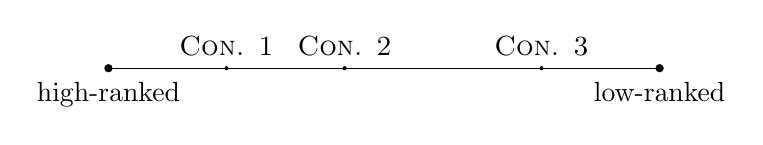
\begin{tikzpicture}
  \draw [circle, inner sep=0pt, minimum size=1.5pt] (0,0) -- +(7,0) ;
  \node[fill, label=below:{high-ranked}, circle, inner sep=0pt, minimum size=3.0pt] (d) at (0,0) {};  
  \node[fill, label=below:{low-ranked}, circle, inner sep=0pt, minimum size=3.0pt] (e) at (7,0) {};    
  \node[fill, label=above:\textsc{Con. 1}, circle, inner sep=0pt, minimum size=1.5pt] (a) at (1.5,0) {};
  \node[fill, label=above:\textsc{Con. 2}, circle, inner sep=0pt, minimum size=1.5pt] (b) at (3.0,0) {};  
  \node[fill, label=above:\textsc{Con. 3}, circle, inner sep=0pt, minimum size=1.5pt] (c) at (5.5,0) {};  
\end{tikzpicture}
\end{figure}

Now, the model has to implement a way to deal with gradient grammaticality, solving the many issues Standard Optimality Theory has with modeling the implicit object construction (debated in \refsec{ot_bad_dobjdrop}). Stochastic Optimality Theory achieves this result by means of the Gradual Learning Algorithm, which is intended to be an improvement on the Constraint Demotion algorithm \parencite{TesarSmolensky1993learnability} used in Standard Optimality Theory. Using the Gradual Learning Algorithm to build a Stochastic Optimality Theoretic grammar is a sensible choice for linguists dealing with any phenomenon where a given input generates candidates with no unique winner, such as language change (with different winners at different times in history), language development (with different winners at different times in the child's life), and complex synchronic phenomena such as indefinite object drop (with different winners at the same time, based on the way constraints interact).\\
Stochastic Optimality Theory allows more than one candidate to be optimal at the same time by allowing constraints to "float" on the continuous scale, as if perturbed by numerical noise at the moment of evaluation. In practice, this is possible by assigning to each constraint a full range of values, centered on what was previously a single point on the scale (now called "ranking value"). Given the range of values, the specific value used at evaluation time is called an "evaluation point". Most importantly, the constraint ranking ranges are defined as probability distributions, and distribution overlap determines the probability of two constraint re-ranking with respect to one another. As illustrated in \reffig{stochot_gaussians1} and \reffig{stochot_gaussians2}, probability distributions in Stochastic Optimality Theory are \textit{normal} distributions. The Gaussian curves are defined by their mean value, which is the ranking value, and their standard deviation, which determines how broad the curve is.\sidenote{Let $\mu$ be the mean value of the distribution and $\sigma$ the standard deviation. The normal distribution is a function defined by the equation:
$$ f(x) = \frac{1}{\sigma\sqrt{2\pi}}e^{-\frac{1}{2}(\frac{x-\mu}{\sigma})^2} $$
} Since all constraints are assigned the same normal distribution in traditional Stochastic Optimality Theory, the actual value of the standard deviation (the "evaluation noise") has no effect on the constraint re-ranking, and it is arbitrarily set at 2 (a different approach to this matter is provided in \textcite{reynolds1994variation, nagy1997optimality}). At evaluation time the selection point will occur most probably in correspondence of the ranking value (given the properties of normal distributions), and its probability steady declines as its value departs from the center of the distribution (i.e., the ranking value).\\
Going back to the simple state of affairs illustrated in \reffig{stot_contranking}, it is evident from \reffig{stochot_gaussians1} that the floating-constraint model makes it now possible for \textsc{Constraint 1} and \textsc{Constraint 2} to re-rank. In the picture, \textsc{Constraint 1} has a ranking value of 6.5 and \textsc{Constraint 2} a ranking value of 4, ordered from the higher-ranked to the lower-ranked as in the custom of Optimality Theory. In particular, as shown by the overlapping curves, the two constraints re-rank freely when the selection points are comprised between 4 and 6.5, and it is much more probable for \textsc{Constraint 1} to outrank \textsc{Constraint 2} than the opposite (graphically, there is only a small area where the curve for \textsc{Constraint 2} is above the curve for \textsc{Constraint 1}, for x values between 4 and 5.25).

\pgfmathdeclarefunction{gauss}{2}{%
  \pgfmathparse{1/(#2*sqrt(2*pi))*exp(-((x-#1)^2)/(2*#2^2))}%
}

\begin{figure}[htb]
\caption{Constraint re-ranking distribution in Stochastic Optimality Theory (overlapping constraints).}
\labfig{stochot_gaussians1}
\begin{tikzpicture}
\begin{axis}[
  no markers, domain=0:10, samples=100, xscale=-1,
  axis lines*=left, xlabel=$x$, ylabel=$y$, 
  every axis y label/.style={at=(current axis.above origin),anchor=south},
  every axis x label/.style={at=(current axis.left of origin),anchor=east},
  height=3cm, width=10cm, % height=5cm, width=12cm,
  xtick={4,6.5}, ytick=\empty,
  enlargelimits=false, clip=false, axis on top,
  grid = major
  ]
  \addplot [fill=cyan!20, draw=none, domain=0:6.5] {gauss(6.5,1)}
  \closedcycle;
  \addplot [fill=cyan!20, draw=none, domain=4:6.5] {gauss(4,1)}
  \closedcycle;
  \addplot [very thick,dotted,cyan!50!black] {gauss(4,1)};
  \addplot [very thick,cyan!50!black] {gauss(6.5,1)};
% \draw [yshift=-1.2cm, latex-latex](axis cs:4,0) -- node [fill=white] {$1.96\sigma$} (axis cs:5.96,0);
\draw [yshift=-0.5cm, latex-latex](axis cs:4,0) -- node [fill=white] {\textsc{Constr. 2}} (axis cs:4,0);
\draw [yshift=-0.5cm, latex-latex](axis cs:6.5,0) -- node [fill=white] {\textsc{Constr. 1}} (axis cs:6.5,0);
\end{axis}
\end{tikzpicture}
\end{figure}

Instead, \textsc{Constraint 2} and \textsc{Constraint 3} never re-rank, since their probability distributions in \reffig{stochot_gaussians2} never overlap (ranking values have been randomly assigned in the picture just for the argument's sake). In situations such as this, the constraint ranking on a continuous scale just reproduces the results of the categorical ranking yielded in standard Optimality Theory, i.e., strict domination.

\begin{figure}[htb]
\caption{Constraint re-ranking distribution in Stochastic Optimality Theory (non-overlapping constraints).}
\labfig{stochot_gaussians2}
\begin{tikzpicture}
\begin{axis}[
  no markers, domain=0:10, samples=100, xscale=-1,
  axis lines*=left, xlabel=$x$, ylabel=$y$,
  every axis y label/.style={at=(current axis.above origin),anchor=south},
  every axis x label/.style={at=(current axis.left of origin),anchor=east},
  height=3cm, width=10cm, % height=5cm, width=12cm,
  xtick={2,8}, ytick=\empty,
  enlargelimits=false, clip=false, axis on top,
  grid = major
  ]
%   \addplot [fill=cyan!20, draw=none, domain=0:5.96] {gauss(8,1)} \closedcycle;
  \addplot [very thick,dotted,cyan!50!black] {gauss(2,1)};
  \addplot [very thick,cyan!50!black] {gauss(8,1)};
% \draw [yshift=-1.2cm, latex-latex](axis cs:2,0) -- node [fill=white] {$1.96\sigma$} (axis cs:5.96,0);
\draw [yshift=-0.5cm, latex-latex](axis cs:2,0) -- node [fill=white] {\textsc{Constr. 3}} (axis cs:2,0);
\draw [yshift=-0.5cm, latex-latex](axis cs:8,0) -- node [fill=white] {\textsc{Constr. 2}} (axis cs:8,0);
\end{axis}
\end{tikzpicture}
\end{figure}

The Gradual Learning Algorithm uses these premises to assign an empirically motivated ranking value to each constraint, modulating its outcome based on an error-driven procedure. The full details of how the algorithm works, which the reader will find in \textcite{BoersmaHayes2001empirical} are outside the scope of this chapter. For the purposes of my dissertation, it is important to note that Stochastic Optimality Theory provides an optimal environment to create a model of object drop. Let us consider a simple example such as \ref{mock_simple_dobj}, where the verb \textit{to eat} is used transitively in \ref{mock_simple_dobj1} and intransitively in \ref{mock_simple_dobj2}, and let us ignore the effect of the many factors influencing object drop (discussed in \refch{factors}) for the time being. Both \ref{mock_simple_dobj1} and \ref{mock_simple_dobj2} are grammatical, but the latter is judged slightly less acceptable than the former on average by some hypothetical native speakers.
% \vspace{-0.5cm} % PER AGGIUSTARE LO SPAZIO PRIMA DEGLI ESEMPI!
\ex. \label{mock_simple_dobj} \a. \label{mock_simple_dobj1} John is eating pizza. \hfill 7
\b. \label{mock_simple_dobj2} John is eating. \hfill 6.5

In our simplified model of object drop, we would posit just two conflicting constraints in the spirit of Optimality Theory (\refsec{classicot}): \textsc{*Internal Argument Structure}, a markedness constraint penalizing the presence of an overt direct object in the output, and \textsc{Faithfulness to Argument Structure}, a faithfulness constraint requiring all the arguments in the input to be also realized in the output. In a standard Optimality Theoretic analysis of the candidate set in \ref{mock_simple_dobj}, \textsc{Faithfulness to Argument Structure} would be ranked above \textsc{*Internal Argument Structure} and make \ref{mock_simple_dobj1} the only winner in the competition, with no reference to the slight acceptability difference. A Stochastic Optimality Theoretic model would solve the problem, so that \textsc{Faithfulness to Argument Structure} would indeed be ranked above \textsc{*Internal Argument Structure} most of the times, but with a large overlap between the two probability distributions (see \reffig{stochot_gaussians_dobj}). Crucially, one constraint outranks the other only probabilistically, while in the standard Optimality Theoretic model it would do so in an absolute sense due to strict domination.

\begin{figure}[htb]
\caption{Constraint re-ranking distribution in Stochastic Optimality Theory relative to Example \ref{mock_simple_dobj}.}
\labfig{stochot_gaussians_dobj}
\begin{tikzpicture}
\begin{axis}[
  no markers, domain=0:10, samples=100, xscale=-1,
  axis lines*=left, xlabel=$x$, ylabel=$y$, 
  every axis y label/.style={at=(current axis.above origin),anchor=south},
  every axis x label/.style={at=(current axis.left of origin),anchor=east},
  height=3cm, width=8cm, % height=5cm, width=12cm,
  xtick={5.5,6.5}, ytick=\empty, xticklabels={,,},
  enlargelimits=false, clip=false, axis on top,
  grid = major
  ]
%   \addplot [fill=cyan!20, draw=none, domain=0:6.5] {gauss(6.5,1)}
%   \closedcycle;
%   \addplot [fill=cyan!20, draw=none, domain=5.5:6.5] {gauss(5.5,1)}
%   \closedcycle;
  \addplot [very thick,dotted,cyan!50!black] {gauss(5.5,1)};
  \addplot [very thick,cyan!50!black] {gauss(6.5,1)};
% \draw [yshift=-1.2cm, latex-latex](axis cs:4,0) -- node [fill=white] {$1.96\sigma$} (axis cs:5.96,0);
\draw [yshift=2.0cm, latex-latex](axis cs:5.5,0) -- node [fill=white] {\textsc{*Int Arg}} (axis cs:5.5,0);
\draw [yshift=-0.5cm, latex-latex](axis cs:6.5,0) -- node [fill=white] {\textsc{Faith Arg}} (axis cs:6.5,0);
\end{axis}
\end{tikzpicture}
\end{figure}

The use of Stochastic Optimality Theory to define a working model of the implicit object construction, aware of the effect of several predictors (\refch{factors}) and the fact that different transitive verbs are differently prone to be used intransitively, is the topic of \refch{medina}.